\subsection{Drone}

\begin{figure}[H]
\centering
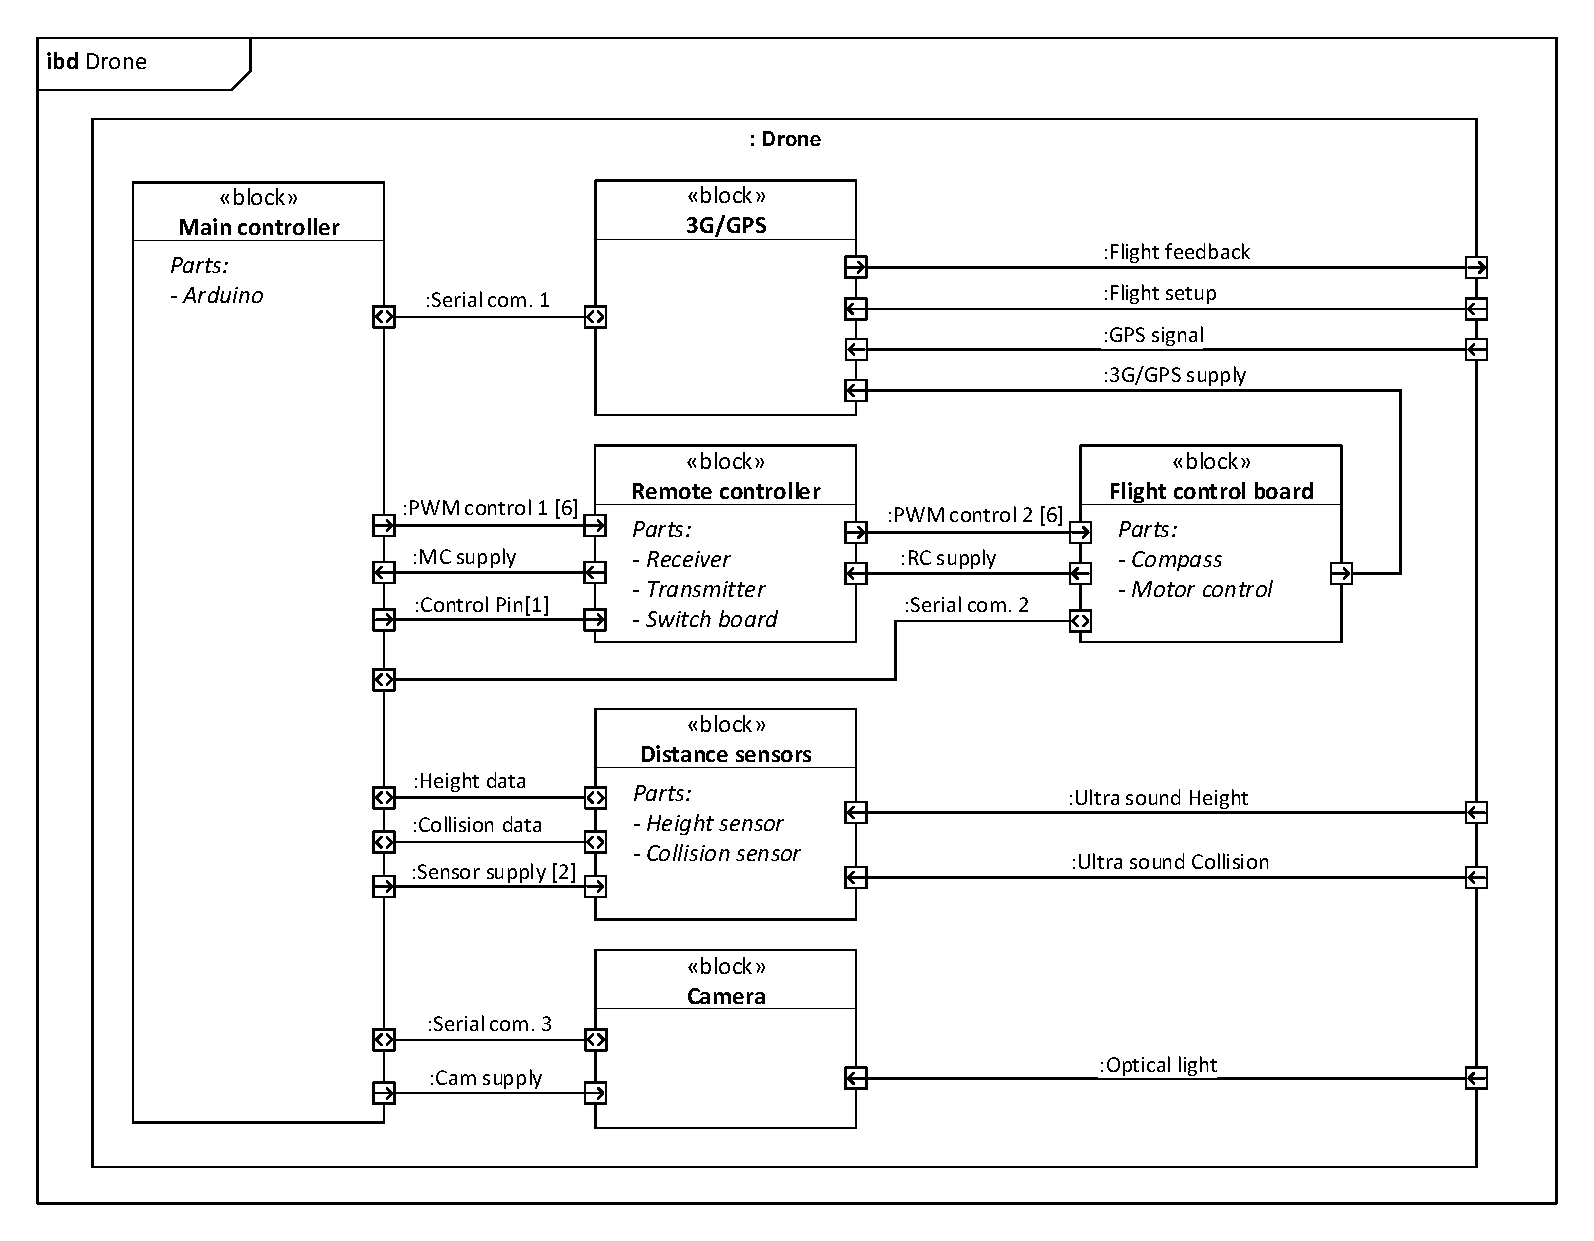
\includegraphics[width=1\textwidth]{Billeder/IBD/ibd2_drone.pdf}
\caption{ibd - drone}
\label{fig:ibd_drone}
\end{figure}

\begin{table}[H]
	\centering
		\begin{tabular}{|p{2.5 cm}|p{5.5 cm}|p{2.5 cm}|p{2.5 cm}|} 
		\hline
			\textbf{Signal navn} 	& \textbf{Signal beskrivelse}		& \textbf{Out} 				& \textbf{In}     \\ \hline
			Serial com. 1		& UART forbindelse & Main controller & 3G/GPS    \\ \hline
			Serial com. 1		& UART forbindelse & Main controller & 3G/GPS    \\ \hline
			3G/GPS supply 		& 3.2 - 4.2 V DC	& Main controller				& 3G/GPS	\\ \hline
			Flight feedback	& & 3G/GPS	& Webapplication	\\ \hline
			
			3G/GPS supply 		& 	& Webapplication				& 3G/GPS	\\ \hline
			Height data.		& Trigger \& echo signal der indikerer afstanden. 	& Main controller.	& Distance sensors.	\\ \hline
			Kollision data.		& Trigger \& echo signal der indikerer afstanden. 	& Main controller.	& Distance sensors.  \\ \hline
			Sensor supply [2]	& 5V DC	& Main controller. & Distance sensors.	\\ \hline
			Serial com. 2		& 	& Main controller				& 	\\ \hline 
			PWM control [6]		& 50 Hz 6 kanals signal.	& Main controller.				& Flight control board.	\\ \hline
			Serial com. 3		& N/A	& Main controller	& Camera	\\ \hline
			Cam supply			& N/A 	& Main controller	& Camera	\\ \hline 
		\end{tabular}
	\caption{Forbindelser til: \textbf{ibd} drone}
	\label{tab:ibddrone}
\end{table}

